\documentclass[14 pt, fleqn]{extarticle}

	\usepackage[frenchb]{babel}
	\usepackage[utf8]{inputenc}  
	\usepackage[T1]{fontenc}
	\usepackage{amssymb}
	\usepackage[mathscr]{euscript}
	\usepackage{stmaryrd}
	\usepackage{amsmath}
	\usepackage{tikz}
	\usepackage[all,cmtip]{xy}
	\usepackage{amsthm}
	\usepackage{varioref}
	\usepackage{geometry}
	\geometry{a4paper}
	\usepackage{lmodern}
	\usepackage{hyperref}
	\usepackage{array}
	 \usepackage{fancyhdr}
	 \usepackage{float}\usepackage{setspace}
\setlength{\mathindent}{1cm}
\renewcommand{\theenumi}{\alph{enumi})}
	\pagestyle{fancy}
	\theoremstyle{plain}
	\fancyfoot[C]{} 
	\fancyhead[L]{}
	\fancyhead[R]{}\geometry{
 a4paper,
 total={170mm,257mm},
 left=5mm,
 top=5mm,
 bottom = 5mm
 }
	
	
	\title{Contrôle}
	\date{}
	\begin{document}
 \subsection*{Exercice 1 (2 + 1 + 1 + 3 + 1 = 8 points) }
 
 \begin{enumerate}
  \item Exprimez le volume d'un cylindre de rayon $3$ cm et de hauteur $5$ cm. Donnez une valeur exacte, et une valeur approchée au mL.
 \item Calculez $(5-3+7-1) + (-9+4-1) - (-3-7+2)$.
 
  \item Supprimez correctement les parenthèses dans 
 $(a-b+c) - (d-e-f) + (b-a)$, puis réduisez l'expression.
  \item Développez et réduisez $2 + x + 4(1-x)$, puis $4 - x + x(1-2x)$.
   \item Réduisez 
 $$ - \frac32x+ \frac54x - 3x^2 + \frac{x}6 - \frac52 x^2 + 5 + 4 x^2.$$
 \end{enumerate}
 
 \subsection*{Exercice 2 (2 + 3 = 5 points)}
 Le capitaine d'un navire possède un trésor constitué de $69$ perles et $1150$ pièces d'or.\begin{enumerate}
\item Décomposer 69 et 1 150 en un produit de facteurs premiers.
\item  Le capitaine partage équitablement le trésor entre les marins. Combien y a-t-il de marins sachant que toutes les pièces et perles ont été distribuées? Que recevra chaque marin?

\end{enumerate}
 
 \subsection*{Exercice 3 (3+3+1 = 7 points)}
 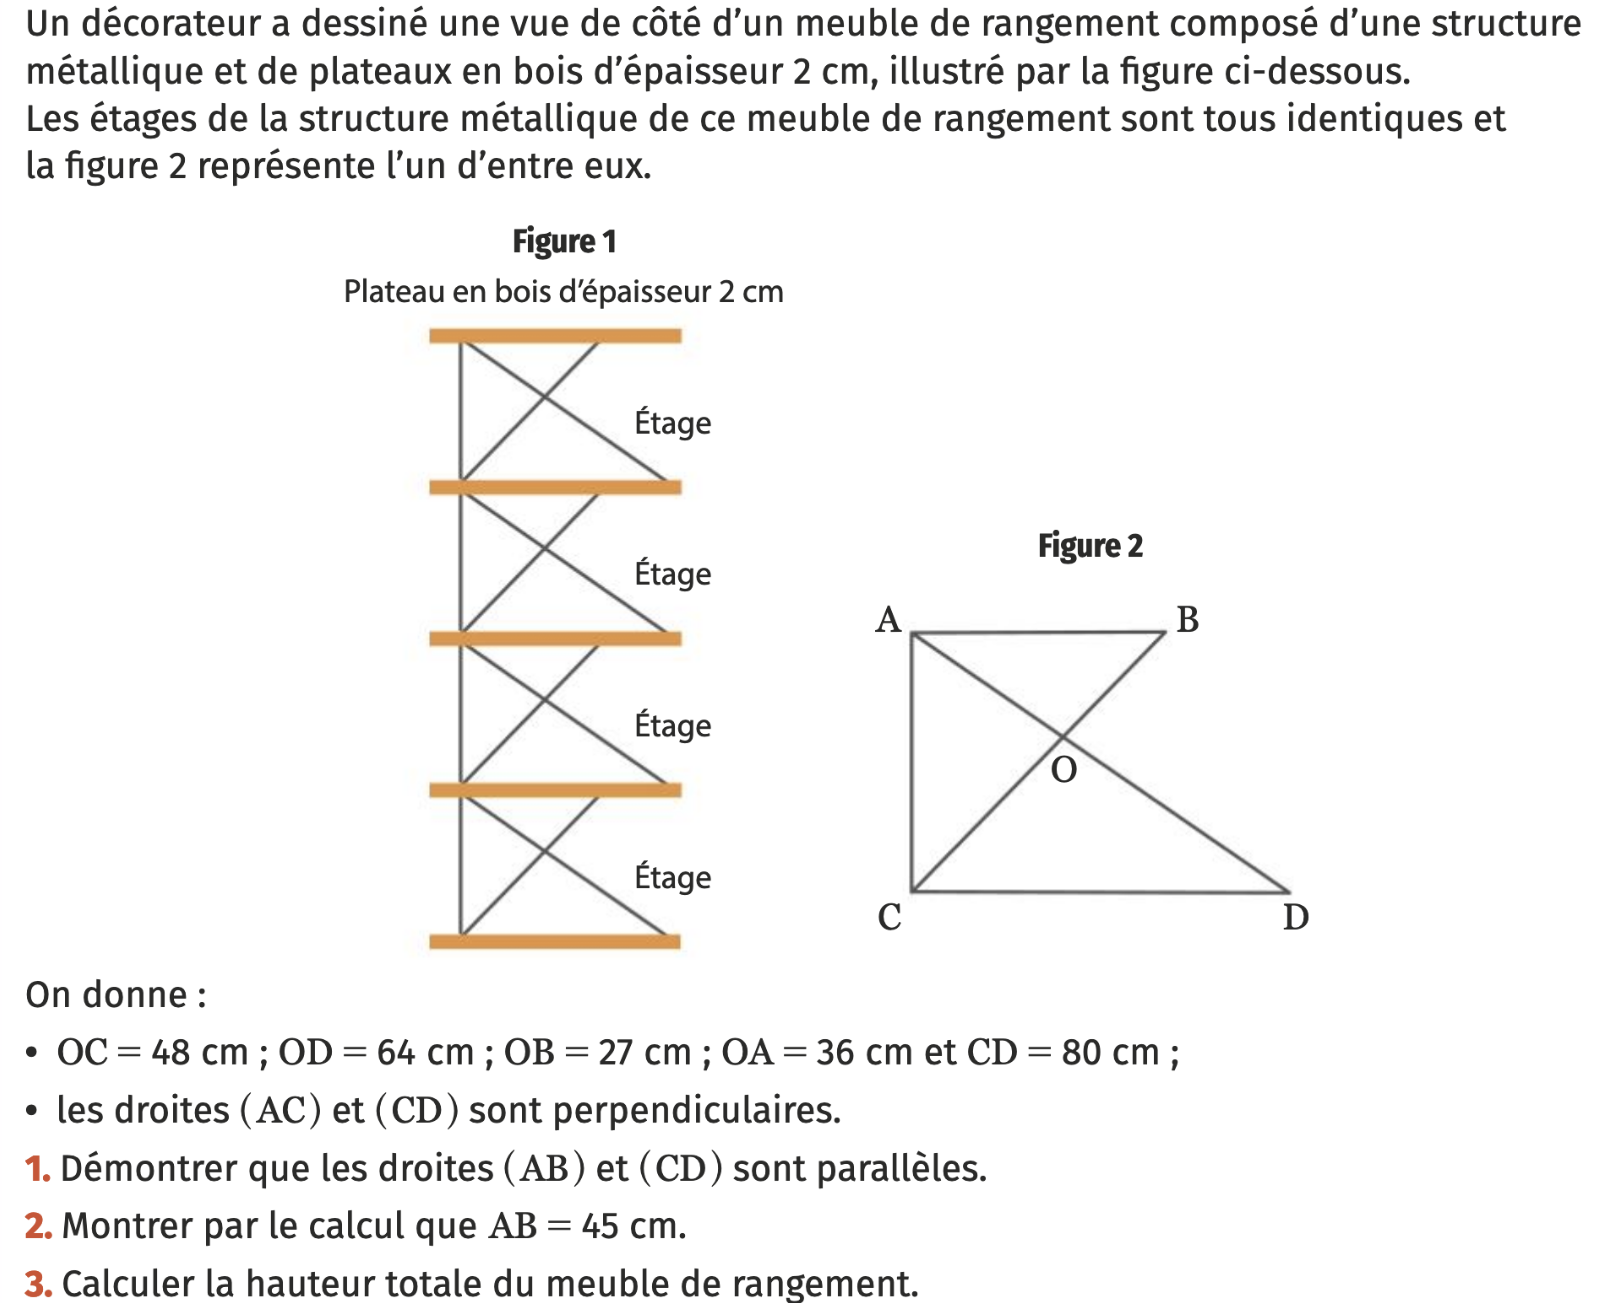
\includegraphics[scale=.6]{Exo}
  
 	\end{document}
